\documentclass[8pt]{beamer}\usepackage[]{graphicx}\usepackage[]{color}
%
% \def\expect#1#2{\underset{#1}{\mathbb{E}}\left[#2\right]}
% \def\sumn{\sum_{n=1}^N}
% \def\x{x}
% \def\xvec{X}
% \def\w{w}
% \def\onevec{1_N}
% \def\infl{\psi}

\usetheme{metropolis}           % Use metropolis theme
\usepackage{amsmath}
\usepackage{tikz}


\usepackage{listings}
\lstset
{
    language=[LaTeX]TeX,
    breaklines=true,
    basicstyle=\tt\scriptsize,
    keywordstyle=\color{blue},
    identifierstyle=\color{magenta},
}

\title{CI introduction}
\author{Ryan Giordano}
\date{Dec 14th, 2021}
\institute{Massachusetts Institute of Technology}

\begin{document}



%%%%%%%%%%%%%%%%%%%%%%%%%%%%%%%%%%%%%%%%%%%%%%%%%%%%%%%%%%%%%%%%%%%%%%%
%%%%%%%%%%%%%%%%%%%%%%%%%%%%%%%%%%%%%%%%%%%%%%%%%%%%%%%%%%%%%%%%%%%%%%%
%%%%%%%%%%%%%%%%%%%%%%%%%%%%%%%%%%%%%%%%%%%%%%%%%%%%%%%%%%%%%%%%%%%%%%%

\begin{frame}[fragile]{Dataset}

Recall our running example from previous classes:\footnotemark[1]



% \begin{center}
% \begin{minipage}{0.38\textwidth}
% %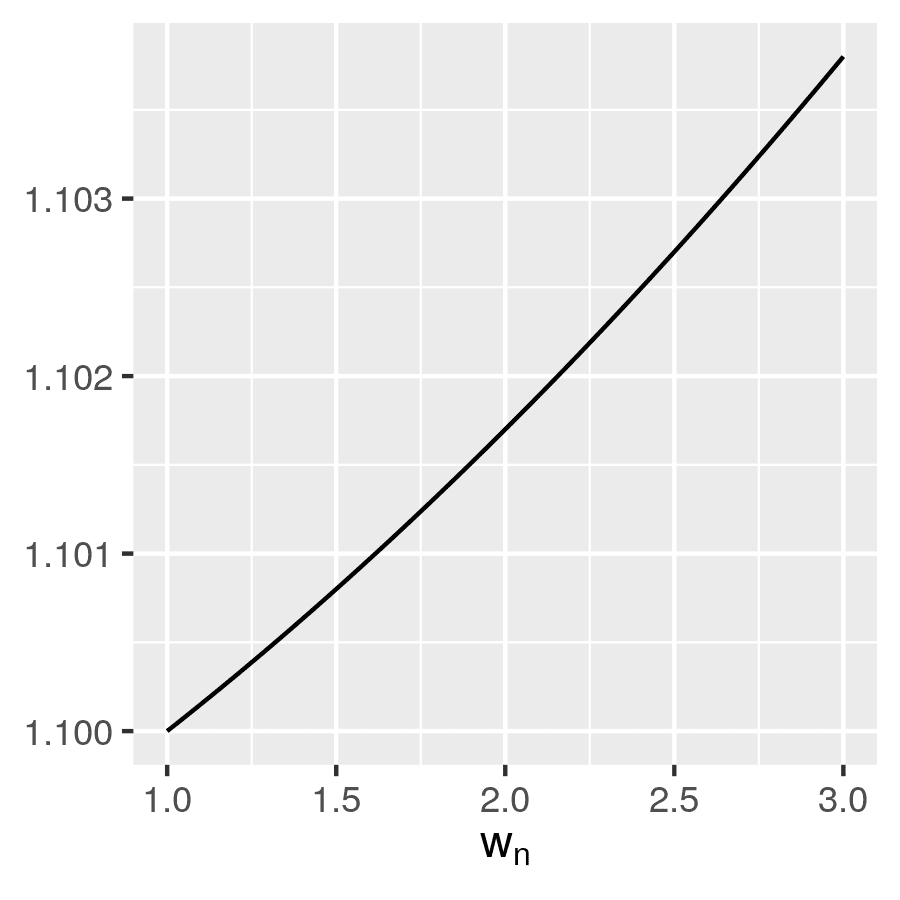
\includegraphics[width=\textwidth]{e_beta_w}
% Hello
% \end{minipage}
% \end{center}

%%%%%%%%%%%%%%%%%%%%%%
\hrulefill

Let's annotate this graphic using TikZ.

\begin{lstlisting}
\begin{center}
\begin{minipage}{0.38\textwidth}
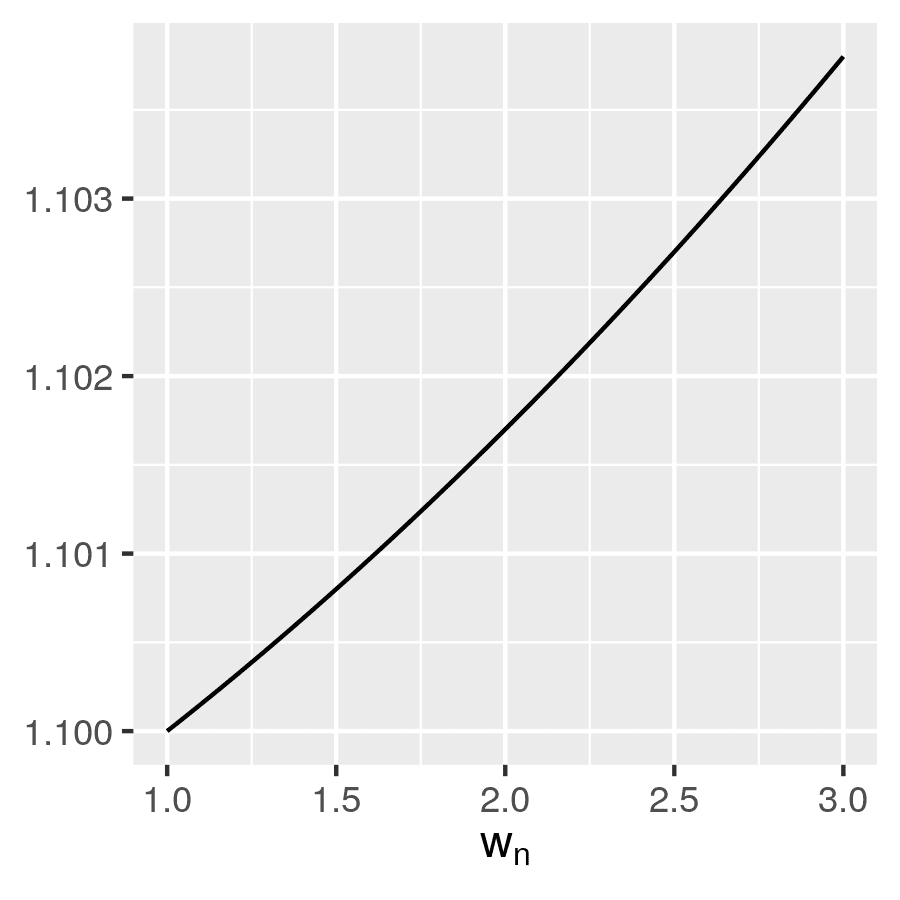
\includegraphics[width=\textwidth]{e_beta_w}
\end{minipage}
\end{center}
\end{lstlisting}

From now on, everything I'm going to do will be within the minipage.

\vfill
\footnotetext[1]{
Taken from Chapter 10 of ``Data Science: A First Introduction'' by
Timbers, Campbell, and Lee
\url{https://ubc-dsci.github.io/introduction-to-datascience/}
}

\end{frame}



\end{document}
